\section{Introduction}
\subsection{Background}
The main social problem we would like to address in this project is menstrual poverty and stigma about women's menstrual circle, also known as period.
According to the “National Plan for the Development of Children in Poverty Areas” published by the General Office of the State Council of the People's Republic of China, there are about 40 million children (about twice the population of New York) living in special hardship areas. Among this population, about 10\% are girls aged 12-16, and thus at minimum 4 million face menstrual poverty. In addition, according to UU Public Welfare's survey of more than 70 schools in poverty areas in 11 provinces and autonomous regions in China, about 5\% of girls who have menstruated do not use sanitary napkins. Behind menstrual poverty are gynecological diseases, psychological problems, and the risk of being out of school and employment. According to the sanitary napkin brand MeBuEri's website, 93\% of Chinese women suffer from non-essential gynecological diseases, of which 63\% are caused by poor-quality sanitary napkins.

\begin{figure}[ht]
    \centering
    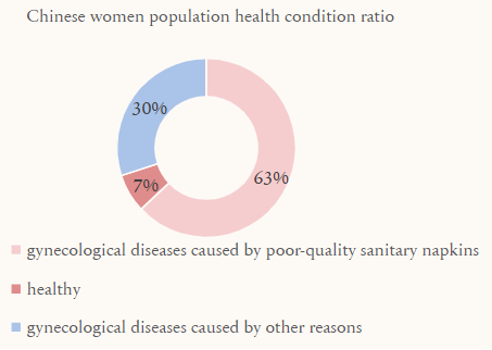
\includegraphics[width=\columnwidth]{assets/napkin_brand.png}
    \caption{According to the sanitary napkin brand MeiBuEr's website, 93\% of Chinese women suffer from non-essential gynecological diseases, of which 63\% are caused by poor-quality sanitary napkins.}
    \label{fig:napkin_brand}
\end{figure}

In trying to persuade our school to provide sanitary napkins, we learned that the budget and responsibility for their delivery in our school are not clear. The logistics department needs more usage to install vending machines for daily necessities like sanitary napkins. The Health Safety Environment department said that sanitary napkins were not first aid supplies and should not be provided in first aid boxes or clinics.\\

In addition, after researching and doing literature reviews of news and reports on related topics, we found that previous attempts to install sharing sanitary napkin self-service boxes in some universities have not been successful. However, personal electronic charging battery banks can be found everywhere in various parks, hotels, and supermarkets. More sanitary napkins are needed in public places.\\

On the other hand, we noticed that family planning supplies such as condoms are available and distributed free of charge in hospitals and clinics. Why do menstrual physiological products that women need for survival are not distributed free of charge? Let alone its importance in preventing gynecological diseases and psychological problems. In China, the news of the demand for sanitary napkin sales on high-speed trains in 2022 became a hot topic on social media. This phenomenon also reflects the attention and urgency of this topic and this service.\\

At the same time, the social stigma against menstrual circles troubles more women. For example, menstruation is still regarded as a shameful thing on many occasions, replaced by euphemism words such as "great aunt" and "that" in conversations. In addition, period products are often deliberately hidden in daily life, such as black plastic bags in convenience stores.\\

From our previous survey among undergraduate students, 43\% of students don't feel comfortable talking about sanitary napkins and periods in public with some specified reasons below. It's worth highlighting that most of the answers (56\%) are related to negative emotions such as shameful, impolite, embarrassing, awkward, and bad. This result shows that period stigma exists in the student population at Hong Kong University of Science and Technology (Guangzhou). In addition, the menstrual shame problem even exists in some of their parents' and previous teachers' communities. This echoes our hypothesis and implies that these women and their descendants will need a longer time to break through their psychological burdens and become independent without social welfare interventions.

\subsection{Purpose and Vision}
It is necessary to make more people aware that sanitary napkins are daily hygiene products like paper towels and call on more people to pay attention to the needs of women. Women should get used to talking about menstrual circles and buying sanitary napkins with dignity and convenience in vending machines in public places.\\

Build a female-friendly and children-friendly society with humanistic care. The provision of free period items with easy access embodies the fundamental principle of equality and dignity of women and is a fundamental human right. \\

We will first set up an emergency feminie product accessible station in the female restroom of maker space at our school HKUST Guangzhou. We plan to run the pilot project for one year. Starting from the Guangzhou campus of HKUST in Nansha District, we will then expand to other cities in the greater bay area such as Shenzhen, Hong Kong, and Dongguan.

\subsection{Scope of the Study}
To narrow down our vision in the project scope, we aim to first sell sanitary napkins via emergency feminie product accessible station and then provide free emergency sanitary napkins once a month after securing sponsorship. \\

In addition to analyzing vending machine IoT systems, our project also has a data visualization map website that locates existing emergency feminie product accessible station. Furthermore, we developed a rating system to evaluate them and plan to develop this into building lesgislation. This is the educational element to alleviate the stigma against menstrual circles.\\

Team members from Info Hub built the website and advised on IoT system. \\

Team member from SEE Thrust advised on potential solar panel usage to replace vending machine battery. \\

Team members from Society Hub secured vending machine sponsorship, collected data, created website content, drafted survey and policy recommendations.

